\documentclass[a4paper, 12pt, english]{article}

% Import packages:
\usepackage[utf8]{inputenc}
\usepackage[english]{babel} % change to english if english
\usepackage{graphicx, color}
\usepackage{parskip} % norwegian sections (skip line)
\usepackage{amsmath}
\usepackage{varioref} % fancy captions
\usepackage[margin=3cm]{geometry} % smaller margins
\usepackage{grffile} % Extended file name support for graphics, allows periods in filenames
\usepackage[small,bf]{caption}
\usepackage{hyperref}
\usepackage{fancyhdr}
\usepackage{parskip}
\usepackage{caption}

% For placeholder text, :D
\usepackage{lipsum}

% Packages for writing algorithms
\usepackage{algpseudocode}
\usepackage{algorithm}

\definecolor{darkgreen}{RGB}{0,135,0}

% Set code stuff:
\usepackage{listings}
\lstset{language=c++} % or python, java, etc...
\lstset{basicstyle=\ttfamily\scriptsize} % \small if short code
\lstset{frame=single} % creates the frame around code
\lstset{title=\lstname} % display name of file, not necessary
\lstset{keywordstyle=\color{red}\bfseries}
\lstset{commentstyle=\color{blue}}
\lstset{stringstyle =\color{darkgreen}}
\lstset{showspaces=false}
\lstset{showstringspaces=false}
\lstset{showtabs=false}
\lstset{breaklines=true}
\lstset{tabsize=4}

% Custom commands:
%\newcommand{\nameOfCommand}[numberOfArguments]{command}
\newcommand{\D}[1]{\ \mathrm{d}#1} % steps in integrals, ex: 4x \D{x} -> 4x dx
\newcommand{\E}[1]{\cdot 10^{#1}}  % exponents, ex: 1.4\E{3} -> 1.4*10^3
\newcommand{\U}[1]{\, \textrm{#1}} % display units prettily, ex: 15.4\U{m} -> 15.4 m
\newcommand{\degree}{\, ^\circ}    % make a degree symbol

\newcommand{\bilde}[3]{
	\begin{figure}[htbp]
		\centering
		\includegraphics[width=\textwidth]{#1}
		\caption{#3 \label{#2}}
	\end{figure}
}
\newcommand{\bildeto}[4]{
	\begin{figure}[htbp]
		\centering
		\includegraphics[width=0.96\textwidth]{#1}
		\includegraphics[width=0.96\textwidth]{#2}
		\caption{#4 \label{#3}}
	\end{figure}
}

% Commands for referencing
\newcommand{\refeq}[1]{(\textcolor{red}{\ref{eq:#1}})} % Red color when referencing equations.
\newcommand{\refig}[1]{\textcolor{blue}{\ref{fig:#1}}} % Blue color when referencing figures.
\newcommand{\reflst}[1]{(\textcolor{red}{\ref{lst:#1}})}
\newcommand{\reftab}[1]{\textcolor{blue}{\ref{tab:#1}}} % Blue color when referencing tables.

% Fancy ruler needed for titlepage
\newcommand{\HRule}{\rule{\linewidth}{0.5mm}}

% Command for most used vectors
\newcommand{\R}{\mathbf{r}}
\newcommand{\V}{\mathbf{v}}
\newcommand{\A}{\mathbf{a}}

% Opening:
\author{Kristoffer Brækken, Vedad Hodzic, Paul Magnus Sørensen-Clark}

% Begin document:
\begin{document}

\begin{titlepage}
    \thispagestyle{empty}
    % Explanation of \\[]-syntax:
% In the square brackets you can define a certain vertical space
% which is inserted in the text. Convenient for fancy formatting.

\begin{center}
    \LARGE University of Oslo\\[1.5cm]
    \Large FYS3150 - Project 4 \\ Computational physics\\[0.5cm]

    \HRule \\[0.4cm]

    % Title of project
    { \huge \bfseries Diffusion of neurotransmitters in the synaptic cleft \\[0.4cm] }

    \HRule \\[1.5cm]

    % Spaces between lines are there for line breaks
    \large Kristoffer Brækken, \emph{jaremikb}

    \large Paul Magnus Sørensen-Clark, \emph{paulms}

    \large Vedad Hodzic, \emph{vedadh}

    \vfill

    {\large \today}
\end{center}

\end{titlepage}

\begin{abstract}
	
Communication in the brain relies heavily on the diffusion of neurotransmitters
across the synaptic cleft, that separates the cell membranes of two cells.
A solution to the diffusion equation can be used to describe this process, so 
we apply three numerical methods for solving the one-dimensional case. A closed
form solution is used to analyze the numerical accuracy of the explicit
forward Euler, and the implicit backward Euler and Crank-Nicolson scheme. It
shows that the explicit forward Euler algorithm yields the most accurate
results at the loss of stability, while the backward case is stable, but with
poor accuracy. The Crank-Nicolson scheme applies both
the explicit forward Euler and the implicit backward Euler, resulting in a
stable method, with an accuracy in between the two Euler schemes.
The implicit Crank-Nicolson scheme is
then preferred in applications where a very small spatial step length is required,
as to avoid compensating with an even smaller temporal step length --- which will
induce a penalty in computation time.

% This was part of the unfinished first draft
%The dominant means of communication between neurons in the brain depend on
%diffusion of signal molecules called \emph{neurotransmitters} across the
%synaptic cleft that separates the cell membranes of two cells. The
%neurotransmitters are released by vesicles in the axon terminal, upon which
%receptors on the postsynaptic side receive the signal. Further insight in this
%process can be helpful within the field of medicine for treating patients that
%suffer from various illnesses caused by impaired communication in the brain.
%
%We will try to simulate the process of diffusion of neurotransmitters across the
%synaptic cleft by solving the diffusion equation. We do the simulation by
%solving the one-dimensional case using three numerical methods, then 
%
%We will however, in our work, mostly consider the differences in numerical
%accuracy between various numerical methods that solve the one-dimensional case.


\end{abstract}

\section{Introduction}
    The purpose of this exercise is to simulate the diffusion of signal
molecules between neurons, both analytically and numerically. These
molecules are transmitted from a presynaptic membrane and captured
by a postsynaptic membrane. The space in between these membranes is
the synaptic cleft, and this is the area we will simulate.

This diffusion of molecules can be described via the diffusion
equation \[ \frac{\partial u}{\partial t} = D\frac{\partial^2
u}{\partial x^2}. \] In order to describe the physical situation
a numerical integration scheme can be implemented.

Solving this particular equation can provide challenges considering
the double spatial derivative on the right hand side. This can be
avoided via clever use of tridiagonal matrices.

The problem is solved via the explicit Forward Euler scheme, the
implicit Backward Euler scheme as well as the implicit Crank
Nicolson scheme. At later stages, an error analysis comparing the
three schemes is included to highlight potential error and to
illustrate areas of stability.

Each integration scheme produces an error and has an area of
stability. When comparing different numerical methods, these two
are key aspects.

A closed form solution to the problem is also found in order to
compare the numerical results and illustrate errors.


\section{Theory}
    To simplify the problem we will approximate this event by assuming
that all movement happens in the same direction, so that we will
only have one spatial dimension plus time. I.e. we are thinking of
the membranes as being infinitely large and parallel, so that on
average, there is no total movement parallel to the membranes, only
parallel to a normal line between them. This approximation is valid
if both membranes are very large and flat compared to the width of
the synaptic cleft.

The spatial direction is called $x$ and time $t$. The position of
the presynaptic membrane is $x=0$ and the postsynaptic membrane is
at $x=1$. The synaptic cleft is the area between, $x \in [0,1]$. We
will not look at discrete signal molecules, but at a floating
density of molecules at a given point. This is a valid
approximation if there are very many molecules. The density at a
given position is called $u(x)$. The presynaptic membrane will
transmit signal molecules in such a way that $u(0)=1$ always. The
postsynaptic membrane absorbs molecules in such a way that $u(1)=0$
always.

At $t=0$ the synaptic cleft is empty, so $u(x)=0$  for $0 < x \leq
1$. When $t > 0$ the cleft will begin to fill up, until it
eventually reaches a steady state $u_s(x)$ where the rate at which molecules
are removed from the system is the same as the rate at which they
are added.

The nature of the movement of the signal molecules, or the flow of the 
moleculels density, is by diffusion, so we will need to solve the diffusion 
equation with the inital and boundary conditions we have discussed so far.


    \subsection{Analytical solution}
    
In order to determine the numerical accuracy of our results, we need to be able
to compare it with a closed form solution. We're interested in finding a
solution for the one-dimensional diffusion equation
%
\begin{equation}
	\frac{\partial u(x,t)}{\partial t} = \frac{\partial^2 u(x,t)}{\partial x^2}
	\ x \in [0,d], \ t > 0,
	\label{eq:diffusioneq}
\end{equation}
%
where $d = 1$, boundary conditions 
%
\begin{align}
	u(0,t) = 1, \hspace{4cm} u(1,t) = 0
	\label{eq:bc}
\end{align}
%
and initial condition 
%
\begin{equation*}
	u(x,0) = 0.
\end{equation*}
%
It is easier to solve such an equation, both numerically and on a closed form,
by the function being zero at both ends. We can achieve this by first finding the
stationary solution, $u_s(x)$. This means that there is no time development of the
function, so \refeq{diffusioneq} transforms to
%
\begin{equation}
	u_s(x) = \frac{\partial^2 u(x,t)}{\partial x^2} = 0.
	\label{eq:stationary}
\end{equation}
%
It is easy to see that for \refeq{stationary} to be fulfilled, our solution must
be on the form
%
\begin{equation*}
	u(x,t) = Ax + B.
\end{equation*}
%
Applying the boundary conditions \refeq{bc} we get
%
\begin{align*}
	u_s(0) &= B = 1
	u_s(1) &= A + 1 = 0, \Rightarrow \ A = -1
\end{align*}
%
which gives us
%
\begin{equation*}
	u_s(x) = 1 - x.
	label{eq:us*}
\end{equation*}
%
We see now that we can define a new function as $v(x) = u(x) - u_s(x)$, which
has boundary conditions and initial condition
%
\begin{equation}
	v(0) = u(0) - u_s(0) = 1 - 1 = 0
	\label{eq:bc0new}
\end{equation}
\begin{equation}
	v(1) = u(1) - u_s(1) = 0 - 0 = 0
	\label{eq:bc1new}
\end{equation}
\begin{equation}
	v(x,0) = u(x,0) - u_s(x) \\
	v(x,0) = x - 1.
	\label{eq:newInitial}
\end{equation}
%
This means that solving the equation
%
\begin{equation*}
	\frac{\partial v(x,t)}{\partial t} = \frac{\partial^2 v(x,t)}{\partial x^2}
\end{equation*}
%
with boundary conditions
%
\begin{equation*}
	v(0,t) = 0, \hspace{4cm} v(1,t) = 0
\end{equation*}
%
gives the same solution as solving \refeq{diffusioneq} with boundary conditions
\refeq{bc}.

We assume the solution $v(x,t)$ is separable, meaning we can write it as
$v(x,t) = F(x)G(t)$.
This gives us
%
\begin{align}
	\frac{\partial F(x)G(t)}{\partial t} &= \frac{\partial^2 F(x)G(t)}{\partial
	x^2} \\
	F(x)G'(t) &= \frac{\partial F'(x)G(t)}{\partial x} \\
	F(x)G'(t) &= F''(x)G(t) \\
	\frac{F''(x)}{F(x)} &= \frac{G'(t)}{G(t)}.
	\label{eq:separate}
\end{align}
%
Since \refeq{separate} needs to be fulfilled for all $x,t$ we require the two
sides being equal to a constant, $-\lambda^2$.
%
\begin{align*}
	\frac{F''(x)}{F(x)} &= -\lambda^2 \\
	F''(x) + \lambda^2F(x) &= 0
	\label{eq:sepF}
\end{align*}
%
\begin{align*}
	\frac{G'(t)}{G(t)} &= -\lambda^2 \\
	G'(t) = -\lambda^2G(t).
	\label{eq:sepG}
\end{align*}
%
The first equation, \refeq{sepF} is a second-order homogeneous linear
differential equation with constant coefficients. We know the solution is on the
form
%
\begin{equation*}
	F(x) = c_1\exp(r_1x) + c_2\exp{r_2x},
	\label{eq:F}
\end{equation*}
%
with $r_1$, $r_2$ being the roots of the auxiliary equation
%
\begin{align*}
	r^2 + \lambda^2 &= 0
	r &= \pm i\lambda.
	\label{eq:roots}
\end{align*}
%
Inserting \refeq{roots} in \refeq{F} gives
%
\begin{align*}
	F(x) &= c_1\exp{i\lambda x} + c_2\exp{-i\lambda x} \\
	F(x) &= c_1\left[ \cos{\lambda x} + i\sin{\lambda x} \right] + c_2\left[
	\cos{\lambda x} - i\sin{\lambda x} \right] \\
	F(x) &= (c_1 + c_2)\cos{\lambda x} + i(c_1 - c_2)\sin{\lambda x} \\
	F(x) &= A\sin{\lambda x} + B\cos{\lambda x}.
\end{align*}
%
The second equation, \refeq{sepG}, is a first order homogeneous ODE with
constant coefficients. We solve it by integrating
%
\begin{align*}
	\frac{\mathrm{d}G(t)}{\mathrm{d}t} &= -\lambda^2 G(t) \\
	\frac{\mathrm{d}G(t)}{G(t)} &= - \lambda^2 dt \\
	\int \frac{1}{G(t)} \ \mathrm{d}G(t) &= -\lambda^2 \int \mathrm{d}t \\
	\ln{G(t)} &= -\lambda^2 t + d_1 \\
	G(t) &= \exp{-\lambda^2 t + d_1} = \exp{d_1}\exp{-\lambda^2 t} \\
	G(t) &= C\exp{-\lambda^2 t}.
\end{align*}
%
We can determine the coefficients $A,B,C$ from the boundary conditions
\refeq{bc0new}, \refeq{bc1new} and initial condition \refeq{newInitial}.
%
\begin{align*}
	v(0,t) = F(0)G(t) &= 0 \\
	BC\exp{-\lambda^2 t} &= 0 \\
	\Rightarrow B = 0 \hspace{4cm} \mathrm{or} \hspace{4cm} C = 0.
\end{align*}
%
The case where $C = 0$ is a trivial case where there is no time development, and
we are not interested in this solution. We let $B = 0$, which gives us
%
\begin{align*}
	v(1,t) = A\sin{\lambda} C\exp{-\lambda^2 t} &= 0
	\Rightarrow \lambda &= n\pi.
\end{align*}
%
One solution of $v(x,t)$ is then
%
\begin{equation*}
	v(x,t) =  D_n\sin{n\pi x}\exp{-n^2\pi^2 t},
\end{equation*}
%
where we have used $A_nC_n = D_n$.
However, there are infinitely many possible values for $n$, which gives us an
infinite number of solutions. Because the diffusion equation is linear, a
superposition of solutions is also a solution for $v(x,t)$, so
%
\begin{equation*}
	\sum\limits_{n=1}^{\infty} D_n\sin{n\pi x}\exp{-n^2\pi^2 t}.
\end{equation*}
%
We determine the coefficients $D_n$ from the initial condition
\refeq{newInitial}
%
\begin{equation*}
	v(x,0) = \sum\limits_{n=1}^{\infty} D_n\sin{n\pi x} = x - 1.
\end{equation*}
%
We recognize that the coefficients $D_n$ are the Fourier coefficients for
$x - 1$. We can then determine $D_n$ from the Fourier sine series
%
\begin{align*}
	D_n &= 2\int\limits_0^1 (x - 1)\sin{n\pi x} \ \mathrm{d}x \\
	&= 2 \int\limits_0^1 \left( x\sin{n\pi x} - \sin{n\pi x} \right) \
	\mathrm{d}x \\
	&= 2 \left( \left[ x(-\cos{n\pi x}\frac{1}{n\pi} \right]\limits_0^1 
	+ \int\limits_0^1\frac{1}{n\pi}\cos{n\pi x} \ \mathrm{d}x - \int\limits_0^1
	\sin{n\pi x} \ \mathrm{d}x \right) \\
	&= 2 \left( -\frac{1}{n\pi}\cos{n\pi} + \frac{1}{n^2\p^2}\left[
		\sin{n\pi x}
	\right]\limits_0^1 + \left[ \frac{1}{n\pi}\cos{n\pi x} \right]\limits_0^1
	\right) \\
	&= 2 \left( \frac{\sin{n\pi}}{n^2\pi^2} - \frac{1}{n\pi} \right) \\
	&= -\frac{2}{n\pi}.
\end{align*}
%
Now that we have found the coefficients $D_n$, we have our solution $v(x,t)$,
and thus we can find $u(x,t)$.
%
\begin{equation*}
	v(x,t) = u(x,t) - u_s(x) \\
	u(x,t) = v(x,t) + u_s(x) \\
	u(x,t) = 1 - x - \sum\limits_{n=1}^{\infty} \frac{2}{n\pi}\sin{n\pi
	x}\exp{-n^2\pi^2 t}.
\end{equation*}
%


\section{Algorithm}
    \subsection{Forward Euler}

With the forward scheme we have
\begin{align*}
    u_t &= u_{xx} \\
    \frac{u(x_i, t_{j+1}) - u(x_i, t_j)}{\Delta t}
    &= \frac{u(x_{i+1}, t_j) - 2u(x_i, t_j) + u(x_{i-1}, t_j)}{\Delta x^2}.
\end{align*}
This we can simply solve for $u(x_i, t_{j+1}$ to get
\begin{align*}
    u(x_i, t_{j+1}) \\
    &= u(x_i, t_j)
    +  \left( u(x_{i+1}, t_j) - 2u(x_i, t_j) + u(x_{i-1}, t_j) \right)
       \frac{\Delta t}{\Delta x^2}.
\end{align*}
Now we can find any point on $u_{j+1}$ independently of each other as long as we know the previous timestep, $u_j$. We can do a simple loop through $u$ to set all the new positions. The endpoints need to be set outside the loop. In this case the endpoints are fixed, so we need to simply not change them. To solve for several time steps this loop can be placed in an outer time loop.
\begin{algorithm}
    \For{j = 1, 2, 3, \cdots}
        \For{i = 2, 3, \cdots , n-2, n-1}
            \State $ u_{new}(x_i, t_{j+1})
                = u(x_i, t_j)
                + \left( u(x_{i+1}, t_j) - 2u(x_i, t_j) + u(x_{i-1}, t_j) \right
                    \frac{\Delta t}{\Delta x^2} $
        \EndFor
        \State $ u = u_{new} $
    \EndFor
\end{algorithm}


\subsection{Backward Euler}


\subsection{Crank-Nicelson}


\section{Results}
    In the following paragraphs, tests on the accuracy for different
combinations of step sizes $\Delta x$ and $\Delta t$ are done. The
solution given by the three integration schemes are then compared
at two strategically chosen time points $t_1$ and $t_2$ so that at
$u(x, t_1)$ the solution is curved but smooth and at $u(x, t_2)$
the solution is approximately linear, close to the stationairy
state.

The test is done for $\Delta x = 1/10$ and $\Delta x = 1/100$.
$\Delta t$ is chosen to be the upper limit decided by the criterium
of stability \[ \alpha = \frac{\Delta t}{\Delta x^2} \leq
\frac{1}{2}. \] For the Crank Nicolson and Backward Euler scheme,
stability will not be decided by this criterium, yet equal grounds
for the simulation will make comparing more meaningful. This gives
the following test cases.

\begin{center}
\begin{tabular}[htbp]{|l|c|c|}
    \hline
    Case & $\Delta x$ & $\Delta t$ \\
    \hline
    \hline
    Case 1 & 1/10 = 0.1 & $1/200 = 5 \cdot 10^{-3}$ \\
    \hline
    Case 2 & 1/100 = 0.01 & $1/20000 = 5 \cdot 10^{-5}$ \\
    \hline
\end{tabular}
\end{center}

Through trial and error, strategic time points were chosen to be
the following.
\begin{align*}
    & t_1 = 0.085 & t_2 = 0.45
\end{align*}
Comparing the solution gave the plots shown in figure
\refig{case1} and \refig{case2}. The lines are overall close
together, yet the Forward Euler scheme seems to separate itself the
most from the other schemes. Because of the tight correlation,
differences are easier to make out on a different scale, as shown
in figure \refig{zoomed_schemes}.

\begin{figure}[htbp]
    \centering
    \includegraphics[width=0.9\textwidth]{plots/schemes_case1_t1.eps}
    \includegraphics[width=0.9\textwidth]{plots/schemes_case1_t2.eps}
    \caption{A comparison of the different integration schemes for
    test case 1 for the two different time points. Above shows for
    $t_1$ while the lower shows for $t_2$.}
    \label{fig:case1}
\end{figure}

\begin{figure}[htbp]
    \centering
    \includegraphics[width=0.9\textwidth]{plots/schemes_case2_t1.eps}
    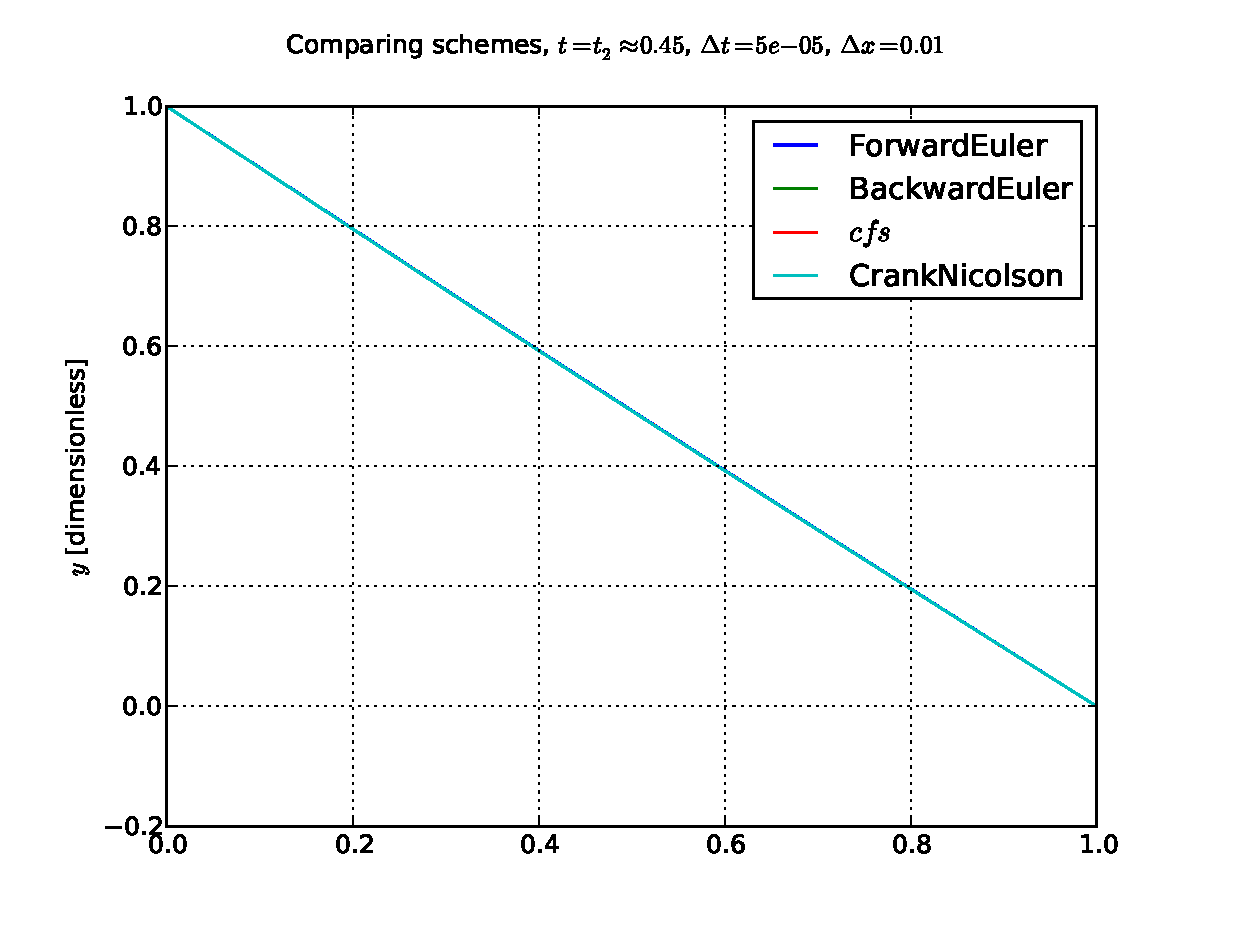
\includegraphics[width=0.9\textwidth]{plots/schemes_case2_t2.eps}
    \caption{A comparison of the different integration schemes for
    test case 2 for the two different time points. Above shows for
    $t_1$ while the lower shows for $t_2$.}
    \label{fig:case2}
\end{figure}

\begin{figure}[htbp]
    \centering
    \includegraphics[width=0.9\textwidth]{plots/schemes_case2_t1_zoomed.eps}
    \caption{A comparison of the different integration schemes for
    test case 2 at $t_1$. Notice the ``zoomed'' in scale in order
    to illustrate differences. The closed form solution lies very
    close to the Crank Nicolson solution.}
    \label{fig:zoomed_schemes}
\end{figure}


    \subsection{Error}
    \bildeto{figures/error_100_0.05_0.1.png}{figures/error_100_1_0.1.png}{fig:error_stable}{$\alpha=0.1$ Forward Euler is well within its stability condition. Top: Before stationairy state. Bottom: After stationairy state.}
\bildeto{figures/error_100_0.05_0.5.png}{figures/error_100_1_0.5.png}{fig:error_limit}{$\alpha=0.5$ Forward Euler is on the edge of being stable. Top: Before stationairy state. Bottom: After stationairy state.}


\section{Discussion}
    Figure \refig{zoomed_schemes} shows that the Forward Euler solution
tends to have higher values than the closed form solution while the
CrankNicolson and Backward Euler schemes tend to have lower values
and lie closer to the closed form.

The idea behind the Forward Euler scheme is to follow the tangent
(the derivative) of the function a predetermined step size, in our
case $\Delta t$. If the derivative tends to have positive values,
this might cause the scheme to approximate values above the closed
form.

Considering the implicit Backward Euler scheme --- this method
might have similar properties causing it to tend to lower values.


    Use results from ex d to say something about why the CN method
seems more exact using among other figure \refig{zoomed_schemes}.


\section{Conclusion}
    This project has discussed different numerical integration schemes
and their area of use. Furthermore the algorithms were implemented
to solve a one dimensional diffusion equation problem.

On account of error and stability analysis, the Crank Nicolson
scheme is observed to produce the least numerical error for the greates span of 
timesteps whilst spanning a greater area of stability compared to its explicit
counterpart and the Backward Euler scheme. If one can afford to have a 
very small timestep the Forward Euler scheme is most accurate, but only then.


\section{Source code}
    \begin{itemize}
    \item jaremikb

        \url{http://www.ulv.no/}
        
    \item paulms

        \url{https://github.com/PaulMag/FYS3150_project4}
        
    \item vedadh

        \url{https://github.com/vedad/Project-4}

\end{itemize}


\end{document}
